\documentclass{scrartcl}
%\documentclass[11pt,english,BCOR10mm,DIV12,bibliography=totoc,parskip=false,smallheadings, headexclude,footexclude,oneside]{pst-doc}

\usepackage[latin1]{inputenc}
\usepackage[compat]{pst-optexp}
\usepackage{pst-func}
\usepackage{pst-circ}
\usepackage{nicefrac}
\usepackage{showexpl}
\makeatletter\renewcommand*\SX@Info{}\makeatother
\lstset{%
  language=PSTricks,
  float=hbp,%
  basicstyle=\ttfamily\small, %
  columns=flexible, %
  tabsize=4, %
  extendedchars=true, %
  showspaces=false, %
  showstringspaces=false, %
  breaklines=true, %
  breakautoindent=true, %
  captionpos=b, %
  xleftmargin=1em, %
  rulecolor=\color{black!20}, %
  explpreset={%
    escapeinside={*}{*}, pos=l, width=-99pt, hsep=5mm, overhang=0pt,
    varwidth, vsep=\bigskipamount, rframe={}}}

\psset{usefiberstyle=true}
\addtopsstyle{Fiber}{linecolor=red,linewidth=1.5\pslinewidth}
\addtopsstyle{Beam}{linewidth=1.5\pslinewidth}
%%%%%%%%%%%%%%%%%%%%%%%%%%%%%%%%%%%%%%%%%%%%%%%%%%%%%%%%%%%%%%%%%%%%%%%%
\begin{document}

\begin{LTXexample}[pos=t, vsep=0.8cm]
\begin{pspicture}[showgrid=true](8,2)
\psset{beam}
\lens[optional](0,1)(3,1){L}
\mirror[showoptdots](4,1)(7,1)(7,0){mirror}
\end{pspicture}
\end{LTXexample}



\begin{LTXexample}[pos=t, vsep=0.8cm]
\begin{pspicture}[showgrid=true](8,2)
  \psset{beam}
  \addtopsstyle{OptComp}{linestyle=dashed, dash=2pt 2pt}
  % wrong, also beam width is changed
  \mirror[linewidth=3\pslinewidth](0,1)(3,1)(3,0){mirror}
  % correct result
  \mirror[addtoOptComp={linewidth=3\pslinewidth}](5,1)(7,1)(7,0){mirror}
\end{pspicture}
\end{LTXexample}



\begin{LTXexample}[width=3.5cm]
\begin{pspicture}[showgrid=true](3,2) 
  \lens[beam, position=0.8](0,1.2)(3,1.2){L}
\end{pspicture}
\end{LTXexample}



\begin{LTXexample}[width=3.5cm]
\begin{pspicture}[showgrid=true](3,2) 
  \lens[beam, abspos=1](0,1.2)(3,1.2){L}
\end{pspicture}
\end{LTXexample}



\begin{LTXexample}[width=5cm]
\begin{pspicture}(-2,-2)(2.5,2)
   \multido{\i=0+45}{8}{%
      \optbox[endbox,
              labelref=relative,
              labeloffset=0,
              optboxwidth=1,
              optboxheight=0.6](0,0)(1;\i){\i}
   }
\end{pspicture}
\end{LTXexample}



\begin{LTXexample}[width=5cm]
\begin{pspicture}(-2,-2)(2.5,2)
   \multido{\i=0+72}{5}{%
      \optbox[endbox,
              labelref=relgrav,
              optboxwidth=1,
              optboxheight=0.6](0,0)(1;\i){\i}
   }
\end{pspicture}
\end{LTXexample}



\begin{LTXexample}[width=5cm]
\begin{pspicture}(-2,-2)(2.5,2)
   \multido{\i=0+72}{5}{%
      \optbox[endbox,
              labelref=global,
              optboxwidth=1,
              optboxheight=0.6](0,0)(1;\i){\i}
   }
\end{pspicture}
\end{LTXexample}



\begin{LTXexample}[width=5cm]
  \begin{pspicture}[showgrid=true](0,0)(3,3)
    \psset{endbox, beam}
    \optbox[label=1 -45](1,0)(2,1){label}
    \optbox[label=0 . . relative](0.6,0.6)(0.6,1.6){label}
  \end{pspicture}
\end{LTXexample}



\begin{LTXexample}[pos=t, vsep=8mm]
\begin{pspicture}[showgrid=true](11,3) 
   \psset{conn=o-o, labelangle=-90, labeloffset=0.3}
   \optbox[extnode=tl](0,2.5)(3,2.5){\texttt{tl}}\psdot(ExtNode)
   \optbox[extnode=l](0,1.5)(3,1.5){\texttt{l}}\psdot(ExtNode)
   \optbox[extnode=bl](0,0.5)(3,0.5){\texttt{bl}}\psdot(ExtNode)
   \optbox[extnode=t](4,2.5)(7,2.5){\texttt{t}}\psdot(ExtNode)
   \optbox[extnode=c](4,1.5)(7,1.5){\texttt{c}}\psdot(ExtNode)
   \optbox[extnode=b](4,0.5)(7,0.5){\texttt{b}}\psdot(ExtNode)
   \optbox[extnode=tr](8,2.5)(11,2.5){\texttt{tr}}\psdot(ExtNode)
   \optbox[extnode=r](8,1.5)(11,1.5){\texttt{r}}\psdot(ExtNode)
   \optbox[extnode=br](8,0.5)(11,0.5){\texttt{br}}\psdot(ExtNode)
\end{pspicture}
\end{LTXexample}



\begin{LTXexample}[width=4.5cm]
\begin{pspicture}[showgrid=true](4,5)
  \addtopsstyle{Beam}{arrows=->, arrowscale=1.5}
  \psset{labeloffset=0}
  \doveprism[conn=o-](0,4.5)(4,4.5){\texttt{o-}}
  \doveprism[conn=i-](0,3.5)(4,3.5){\texttt{i-}}
  \doveprism[conn=-o](0,2.5)(4,2.5){\texttt{-o}}
  \doveprism[conn=-i](0,1.5)(4,1.5){\texttt{-i}}
  \optbox[conn=-f](0,0.5)(4,0.5){\texttt{-f}}
\end{pspicture}
\end{LTXexample}



\begin{LTXexample}[width=4.5cm]
\begin{pspicture}[showgrid=true](4,5)
   \pnode(1,1){A}\pnode(1,4){G}\pnode(3,4){B}
   \optbox[endbox, labelref=relative, labeloffset=0, optboxwidth=1](G)(A){Laser}
   \lens[lens=0.5 0.5 0.5, abspos=0.3](A)(G){}
   \pinhole[abspos=0.5](A)(G){}
   \lens[lens=2, abspos=0.8](A)(G){}
   \lens[abspos=2, labelangle=180](A)(G){L}
   \optplate[abspos=1.5, labeloffset=1](A)(G){SLM}
   \lens[abspos=1](G)(B){L}
   \optbox[endbox, labeloffset=0, optboxwidth=1](G)(B){CCD}
   \pentaprism[beam, labeloffset=1](A)(G)(B){PP}
\end{pspicture}
\end{LTXexample}


\begin{LTXexample}[width=4.5cm]
    \begin{pspicture}[showgrid=true](4,6) \psset{labeloffset=0.6}
      \addtopsstyle{Beam}{arrows=->, arrowscale=1.5}
      \doveprism[compname=Dove1](0,0.8)(3,0.8){Dove1}
      \drawbeam[conn=b-]{Dove1}{(3,0.8)}
      \doveprism[compname=Dove2](0,2.3)(3,2.3){Dove2}
      \drawbeam[conn=B-]{Dove2}{(3,2.3)}
      \doveprism[compname=Dove3](0,3.8)(3,3.8){Dove3}
      \drawbeam[conn=-a]{(0,3.8)}{Dove3}
      \doveprism[compname=Dove4](0,5.3)(3,5.3){Dove4}
      \drawbeam[conn=-A]{(0,5.3)}{Dove4}
    \end{pspicture}
  \end{LTXexample}


\begin{LTXexample}[width=4.5cm]
\begin{pspicture}[showgrid=true](4,6)
   \pnode(1,1){A}\pnode(1,5){G}\pnode(3,5){B}
   \optbox[endbox, labelref=relative, labeloffset=0, optboxwidth=1](G)(A){Laser}
   \lens[lens=0.5 0.5 0.5, abspos=1.5](A)(G){}
   \pinhole[abspos=1.7](A)(G){}
   \lens[lens=2, abspos=2](A)(G){}
   \lens[abspos=3, labelangle=180](A)(G){L}
   \optplate[abspos=2.5, labeloffset=1](A)(G){SLM}
   \lens[abspos=1](G)(B){L}
   \optbox[endbox, labeloffset=0, optboxwidth=1](G)(B){CCD}
   \optdiode[abspos=0.8, conn=o-, compname=OD](A)(G){OD}
   \addtopsstyle{Beam}{linecolor=blue}
   \pentaprism[conn=-i, labeloffset=1, compname=PP](A)(G)(B){PP}
   \addtopsstyle{Beam}{linecolor=red}
   \drawbeam[conn=b-a]{OD}{PP}
\end{pspicture}
\end{LTXexample}


\begin{LTXexample}[width=5.5cm]
\begin{pspicture}[showgrid=true](5,6)
  % concave lenses
  \pnode(0,5){A}\pnode(5,5){B}
  \psline[style=Beam](A)(B)
  \lens[position=0.2](A)(B){L}
  \lens[lensradius=-1,position=0.5](A)(B){L}
  \lens[lens=-1.5 1,position=0.7](A)(B){L}
  % convex lenses
  \pnode(0,3){A}\pnode(5,3){B}
  \psline[style=Beam](A)(B)
  \lens[position=0.2,lens=1 -1](A)(B){L}
  \lens[lens=0 -1](A)(B){L}
  \lens[lens=1 0,position=0.7](A)(B){L}
  % thick lenses
  \pnode(0,1){A}\pnode(5,1){B}
  \psline[style=Beam](A)(B)
  \lens[position=0.3, lens=-1.5 1 1 0.5, thicklens](A)(B){thicklens}
  \lens[lens=0 -1, position=0.7, fillstyle=solid, fillcolor=blue!30!white](A)(B){lens}
\end{pspicture}
\end{LTXexample}



\begin{LTXexample}[width=3.5cm]
\begin{pspicture}[showgrid=true](3,2)
  \optplate[beam](0,1.2)(3,1.2){filter}
\end{pspicture}
\end{LTXexample}



\begin{LTXexample}[width=3.5cm]
\begin{pspicture}[showgrid=true](3,2)
  \optplate[angle=10, beam](0,1.2)(3,1.2){glass plate}
\end{pspicture}
\end{LTXexample}



\begin{LTXexample}[width=3.5cm]
\begin{pspicture}[showgrid=true](3,2)
  \pnode(0,1.2){A}
  \pnode(3,1.2){B}
  \optretplate[beam](A)(B){$\nicefrac{\lambda}{2}$}
\end{pspicture}
\end{LTXexample}



\begin{LTXexample}[width=3.5cm]
\begin{pspicture}[showgrid=true](3,2)
  \pnode(0,1.2){A}
  \pnode(3,1.2){B}
  \pinhole[beam](A)(B){PH}
\end{pspicture}
\end{LTXexample}



\begin{LTXexample}[width=3.5cm]
\begin{pspicture}[showgrid=true](3,2)
  \pnode(0,1.2){A}
  \pnode(3,1.2){B}
  \crystal[fillstyle=solid, fillcolor=yellow!90!black, labelangle=-45, labeloffset=1.2, voltage, lamp, beam](A)(B){SBN:Ce}
\end{pspicture}
\end{LTXexample}



\begin{LTXexample}[width=3.5cm]
\begin{pspicture}[showgrid=true](3,2)
  \optbox[beam](0,0)(3,2){box}
\end{pspicture}
\end{LTXexample}



\begin{LTXexample}[width=3.5cm]
\begin{pspicture}[showgrid=true](3,2)
  \optbox[beam, endbox](0,0)(1.7,1){box}
\end{pspicture}
\end{LTXexample}



\begin{LTXexample}[width=3.5cm]
\begin{pspicture}[showgrid=true](3,2)
  \pnode(0,0){A}
  \pnode(1.7,1){B}
  \optbox[beam, endbox, labelref=relative, labeloffset=0](A)(B){box}
\end{pspicture}
\end{LTXexample}



\begin{LTXexample}[width=3.5cm]
\begin{pspicture}[showgrid=true](3,2)
  \optbox[angle=20, beam, rotateref=l, labeloffset=0.5](0,1)(3,1){box}
\end{pspicture}
\end{LTXexample}



\begin{LTXexample}[width=3.5cm]
\begin{pspicture}[showgrid=true](3,2)
  \pnode(0,1){A}
  \pnode(3,1){B}
  \optbox[labeloffset=0.7, optboxwidth=0.5, optboxheight=1, angle=20, refractiveindex=2.3, compname=Box](A)(B){glass plate}
  \drawbeam[conn=-a]{(A|BoxIntern1)}{Box}
  \drawbeam[conn=B-]{Box}{(B|BoxInternN)}
\end{pspicture}
\end{LTXexample}



\begin{LTXexample}[width=3.5cm]
\begin{pspicture}[showgrid=true](3,2)
  \pnode(0,0){A}
  \pnode(1.7,1){B}
  \optdetector[beam](A)(B){detector}
\end{pspicture}
\end{LTXexample}



\begin{LTXexample}[width=3.5cm]
\begin{pspicture}[showgrid=true](3,2)
  \pnode(0,0){A}
  \pnode(1.7,1){B}
  \optdetector[beam, dettype=diode](A)(B){detector}
\end{pspicture}
\end{LTXexample}



\begin{LTXexample}[width=3.5cm]
\begin{pspicture}[showgrid=true](3,2)
   \optdiode[conn=o-o](0,1)(3,1){Diode}
\end{pspicture}
\end{LTXexample}



\begin{LTXexample}[width=3.5cm]
\begin{pspicture}[showgrid=true](3,2)
  \doveprism[beam](0,1)(3,1){Dove}
\end{pspicture}
\end{LTXexample}



\begin{LTXexample}[width=3.4cm]
\begin{pspicture}[showgrid=true](3,5)
  \pnode(0,0.5){A1}\pnode(3,0.5){B1}\pnode(0,1.5){A2}
  \pnode(3,1.5){B2}\pnode(0,2.5){A3}\pnode(3,2.5){B3}
  \pnode(0,3.5){A4}\pnode(3,3.5){B4}\pnode(0,4.5){A5}
  \pnode(3,4.5){B5}\psset{style=Beam}
  \multido{\i=1+1}{5}{\psline(A\i)(B\i)}
  \psset{linecolor=black}
  \polarization[poltype=misc,position=0.2](A5)(B5)
  \polarization[poltype=perp,position=0.35](A4)(B4)
  \polarization[poltype=parallel,position=0.5](A3)(B3)
  \polarization[poltype=rcirc,position=0.65](A2)(B2)
  \polarization[poltype=lcirc,position=0.8](A1)(B1)
\end{pspicture}
\end{LTXexample}



\begin{LTXexample}[width=3.5cm]
\begin{pspicture}[showgrid=true](3,3)
  \pnode(0,0){A}
  \pnode(1.8,2.2){G}
  \pnode(0,3){B}
  \mirror[beam](A)(G)(B){mirror}
\end{pspicture}
\end{LTXexample}



\begin{LTXexample}[width=3.5cm]
\begin{pspicture}[showgrid=true](3,3)
  \pnode(0,0){A}
  \pnode(1.8,2.2){G}
  \pnode(0,3){B}
  \mirror[beam, variable](A)(G)(B){M$_\mathrm{var}$}
\end{pspicture}
\end{LTXexample}



\begin{LTXexample}[width=3.5cm]
\begin{pspicture}[showgrid=true](3,3)
  \pnode(0,0){A}
  \pnode(1.8,2.2){G}
  \pnode(0,3){B}
  \mirror[beam, mirrortype=piezo,labelangle=-90](A)(G)(B){piezo}
\end{pspicture}
\end{LTXexample}



\begin{LTXexample}[width=3.5cm]
\begin{pspicture}[showgrid=true](3,3)
  \pnode(0,0){A}
  \pnode(1.8,2.2){G}
  \pnode(0,3){B}
  \mirror[beam, mirrortype=extended](A)(G)(B){M$_\mathrm{ext}$}
\end{pspicture}
\end{LTXexample}



\begin{LTXexample}[width=3.5cm]
\begin{pspicture}[showgrid=true](3,3)
  \pnode(0,0){A}\pnode(1,2){G1}
  \pnode(1.8,1){G2}\pnode(2.5,3){B}
  \psset{labeloffset=0.5}
  \psline[style=Beam](A)(G1)(G2)(B)
  \mirror[mirrortype=extended, mirrorradius=1](A)(G1)(G2){M$_{\mathrm{concave}}$}
  \mirror[mirrorradius=-1](G1)(G2)(B){M$_{\mathrm{convex}}$}
\end{pspicture}
\end{LTXexample}



\begin{LTXexample}[width=3.5cm]
\begin{pspicture}[showgrid=true](3,3)
  \pnode(0,2){A}
  \pnode(2,2){G}
  \pnode(3,0){B}
  \beamsplitter[beam](A)(G)(B){BS}
\end{pspicture}
\end{LTXexample}



\begin{LTXexample}[width=3.5cm]
\begin{pspicture}[showgrid=true](3,3)
  \pnode(0,2){A}
  \pnode(2,2){G}
  \pnode(3,0){B}
  \beamsplitter[bsstyle=plate, beam](A)(G)(B){BS}
\end{pspicture}
\end{LTXexample}



\begin{LTXexample}[width=3.5cm]
\begin{pspicture}[showgrid=true](3,3)
  \pnode(0,3){A}
  \pnode(1.8,2.2){G}
  \pnode(0,0){B}
  \optgrid[beam](A)(G)(B){grid}
\end{pspicture}
\end{LTXexample}



\begin{LTXexample}[width=3.5cm]
\begin{pspicture}[showgrid=true](3,3)
  \pnode(0,3){A}
  \pnode(1.8,2.2){G}
  \pnode(0,0){B}
  \optgrid[beam, reverse](A)(G)(B){grid}
\end{pspicture}
\end{LTXexample}



\begin{LTXexample}[width=3.5cm]
\begin{pspicture}[showgrid=true](3,3)
  \pnode(0,3){A}
  \pnode(1.8,2.2){G}
  \pnode(0,0){B}
  \optgrid[beam,%
           optgridcount=6,%
           optgriddepth=0.2,%
           optgridheight=0.3](A)(G)(B){grid}
\end{pspicture}
\end{LTXexample}



\begin{LTXexample}[width=3.5cm]
\begin{pspicture}[showgrid=true](3,3)
  \pnode(0,3){A}
  \pnode(1.8,2.2){G}
  \pnode(0,0){B}
  \optgrid[beam, optgridtype=binary](A)(G)(B){grid}
\end{pspicture}
\end{LTXexample}



\begin{LTXexample}[width=3.5cm]
\begin{pspicture}[showgrid=true](3,3)
  \pnode(0,2.5){A}
  \pnode(2,2){G}
  \pnode(3,0){B}
  \optprism[beam](A)(G)(B){Prism}
\end{pspicture}
\end{LTXexample}



\begin{LTXexample}[width=3.5cm]
\begin{pspicture}[showgrid=true](3,2)
  \pnode(0,1.5){A}
  \pnode(1.8,0.8){G}
  \pnode(0,0.5){B}
  \rightangleprism[beam, showoptdots](A)(G)(B){RA}
\end{pspicture}
\end{LTXexample}



\begin{LTXexample}[width=3.5cm]
\begin{pspicture}[showgrid=true](3,3)
  \pnode(0,2){A}
  \pnode(2,2){G}
  \pnode(2,0){B}
  \pentaprism[beam](A)(G)(B){PP}
\end{pspicture}
\end{LTXexample}



\begin{LTXexample}[width=3.5cm]
\begin{pspicture}[showgrid=true](3,3)
  \pnode(0,2){A}
  \pnode(3,1){B}
  \optdipole[labeloffset=1, beam](A)(B){%
    \rput(0,0){%
      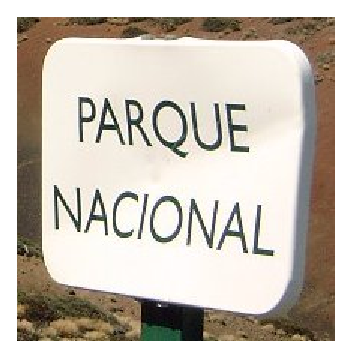
\includegraphics[scale=0.25]{parque-nacional}
    }
  }{label}
\end{pspicture}
\end{LTXexample}



\begin{LTXexample}[width=3.5cm]
\begin{pspicture}[showgrid=true](3,3)
  \pnode(0,0){A}
  \pnode(1.5,2){G}
  \pnode(3,1.5){B}
  \opttripole[beam](B)(G)(A){\rput[b](0,0){text}}{label}
\end{pspicture}
\end{LTXexample}



\begin{LTXexample}[width=3.5cm]
\begin{pspicture}[showgrid=true](3,2)
  \optfiber[labeloffset=0.4](0,1)(3,1){SSMF}
\end{pspicture}
\end{LTXexample}



\begin{LTXexample}[width=3.5cm]
\begin{pspicture}[showgrid=true](3,2)
  \optamp(0,1)(3,1){EDFA}
\end{pspicture}
\end{LTXexample}



\begin{LTXexample}[width=3.5cm]
\begin{pspicture}[showgrid=true](3,2)
  \optmzm(0,1)(3,1){MZM}
\end{pspicture}
\end{LTXexample}



\begin{LTXexample}[width=3.5cm]
\begin{pspicture}[showgrid=true](3,2)
  \optfilter(0,1)(3,1){bandpass}
\end{pspicture}
\end{LTXexample}



\begin{LTXexample}[width=3.5cm]
\begin{pspicture}[showgrid=true](3,2)
  \optfilter[filtertype=bandstop](0,1)(3,1){bandstop}
\end{pspicture}
\end{LTXexample}



\begin{LTXexample}[width=3.5cm]
\begin{pspicture}[showgrid=true](3,2)
  \polcontrol(0,1)(3,1){PC}
\end{pspicture}
\end{LTXexample}



\begin{LTXexample}[width=3.5cm]
\begin{pspicture}[showgrid=true](3,2)
  \optisolator(0,1)(3,1){}
\end{pspicture}
\end{LTXexample}



\begin{LTXexample}[width=3.5cm]
\begin{pspicture}[showgrid=true](3,2)
  \optswitch(0,1)(3,1){Opened switch}
\end{pspicture}
\end{LTXexample}



\begin{LTXexample}[width=3.5cm]
\begin{pspicture}[showgrid=true](3,2)
  \optswitch[switchstyle=closed](0,1)(3,1){Closed switch}
\end{pspicture}
\end{LTXexample}



\begin{LTXexample}[width=3.5cm]
\begin{pspicture}[showgrid=true](3,2)
  \fiberdelayline(0,1)(3,1){Delay line}
\end{pspicture}
\end{LTXexample}



\begin{LTXexample}[width=3.5cm]
\begin{pspicture}[showgrid=true](3,2)
  \optfiberpolarizer(0,1)(3,1){polarizer}
\end{pspicture}
\end{LTXexample}



\begin{LTXexample}[width=3.5cm]
\begin{pspicture}[showgrid=true](3,2)
   \fibercollimator(0.5,1)(2.5,1){FC}
\end{pspicture}
\end{LTXexample}



\begin{LTXexample}[width=3.5cm]
\begin{pspicture}[showgrid=true](3,2)
   \fibercollimator(0,1)(2,1)(3,2){FC}
\end{pspicture}
\end{LTXexample}



\begin{LTXexample}[width=3.5cm]
\begin{pspicture}[showgrid=true](3,2)
   \fibercollimator(0.5,1)(2.5,1)(2.5,2){FC}
\end{pspicture}
\end{LTXexample}



\begin{LTXexample}[width=3.5cm]
\begin{pspicture}[showgrid=true](3,2)
   \fibercollimator[position=0.2](0.5,1)(2.5,1)(2.5,2)(0.5,2){FC}
\end{pspicture}
\end{LTXexample}



\begin{LTXexample}[width=3.5cm]
\begin{pspicture}[showgrid=true](3,2)
  \optcoupler(0.5,2)(0,0.5)(3,1.5)(2.5,0){Coupler}
\end{pspicture}
\end{LTXexample}



\begin{LTXexample}[width=3.5cm]
\begin{pspicture}[showgrid=true](3,2)
  \optcoupler[align=top](0.5,2)(0,0.5)(3,1.5)(2.5,0){Coupler}
\end{pspicture}
\end{LTXexample}



\begin{LTXexample}[width=3.5cm]
\begin{pspicture}[showgrid=true](3,2)
  \optcoupler[align=bottom, couplertype=none](0.5,2)(0,0.5)(3,1.5)(2.5,0){Coupler}
\end{pspicture}
\end{LTXexample}



\begin{LTXexample}[width=3.5cm]
\begin{pspicture}[showgrid=true](3,2)
  \wdmcoupler[labeloffset=0.5](0,1.5)(0,0.5)(3,1){WDM}
\end{pspicture}
\end{LTXexample}



\begin{LTXexample}[width=3.5cm]
\begin{pspicture}[showgrid=true](3,2)
  \newpsstyle{FiberOut2}{style=Fiber, arrows=->}
  \wdmsplitter[align=top, labeloffset=0.5](0,1.5)(3,1.5)(3,0.5){}
\end{pspicture}
\end{LTXexample}



\begin{LTXexample}[width=3.5cm]
\begin{pspicture}[showgrid=true](3,3)
   \addtopsstyle{FiberIn}{ArrowInside=->, arrowscale=1.2}
   \addtopsstyle{FiberOut2}{linecolor=blue}
   \optcoupler(0,2.5)(0,0.5)(3,2.5)(3,0.5){50~\%}
\end{pspicture}
\end{LTXexample}



\begin{LTXexample}[width=3.5cm]
\begin{pspicture}[showgrid=true](3,2)
   \newpsobject{mywdmsplitter}{wdmsplitter}{addtoFiberOut1={arrows=->, arrowscale=1.3, linecolor=blue}, labelangle=180, align=bottom}
   \mywdmsplitter(0,0.5)(3,1.5)(3,0.5){blue band}
\end{pspicture}
\end{LTXexample}



\begin{LTXexample}[width=3.5cm]
\begin{pspicture}[showgrid=true](3,2)
   \newpsobject{mycoupler}{optcoupler}{addtoFiberIn2={angleA=90}, align=top}
   \mycoupler(0.5,1.5)(0.5,0.5)(2.5,1.5)(2.5,0.5){}
\end{pspicture}
\end{LTXexample}



\begin{LTXexample}[width=3.5cm]
\newpsobject{sbn}{crystal}{voltage, lamp, labelangle=45, labeloffset=1.2, fillstyle=solid, fillcolor=yellow!90!black}
\begin{pspicture}[showgrid=true](3,2) 
   \sbn(0,1)(3,1){SBN:Ce}
   \psline[style=Beam](0,1)(3,1)
\end{pspicture}
\end{LTXexample}



\begin{LTXexample}[width=3.5cm]
\newpsobject{pumpcoupler}{wdmcoupler}{align=top, labelangle=180, labeloffset=0.5,addtoFiberIn2={ArrowInside=->, arrowscale=2}}
\begin{pspicture}[showgrid=true](3,2) 
   \pumpcoupler(0,1)(0,0)(3,1){Pumpcoupler}
\end{pspicture}
\end{LTXexample}



\begin{LTXexample}[width=5.5cm]
\newpsobject{MOLensIn}{lens}{lens=0.5 0.5 0.5}
\newpsobject{MOLensOut}{lens}{lens=1.5 1.5 1.5}
\begin{pspicture}[showgrid=true](5,2) 
   \pnode(0,1){A}\pnode(5,1){B}
   \MOLensIn[abspos=0.5](A)(B){}
   \MOLensOut[abspos=1](A)(B){}
   \MOLensOut[abspos=4](A)(B){}
   \MOLensIn[abspos=4.5](A)(B){}
   \psline[style=Beam](A)(B)
\end{pspicture}
\end{LTXexample}


\begin{LTXexample}[width=4.5cm]
\newOptexpTripole{mygrid}{subgriddiv=5, griddots=0, subgridwidth=\pslinewidth, gridwidth=2\pslinewidth}
\makeatletter
\def\mygrid@iii{% put here all PSTricks drawing code
  \psgrid(-1,0)(1,1)
}%
\makeatother
\begin{pspicture}[showgrid=true](4,4) 
   \pnode(0,1){A}\pnode(2,2){G}\pnode(3,0){B}
   \mygrid[gridcolor=red,labeloffset=1.5](A)(G)(B){myGrid}
   \psline[style=Beam](A)(G)(B)
\end{pspicture}
\end{LTXexample}


\begin{LTXexample}[pos=t,vsep=8mm]
\begin{pspicture}(10,2)
\psset{optboxwidth=1}\addtopsstyle{Beam}{linewidth=2\pslinewidth}
\pnode(1,1){Start}\pnode(9,1){CCD}\optbox[endbox, labeloffset=0](CCD)(Start){Laser}
\optbox[endbox,labeloffset=0,beam](Start)(CCD){CCD}
\polarization[poltype=perp,abspos=0.5](Start)(CCD)
\optretplate[abspos=1](Start)(CCD){$\nicefrac{\lambda}{2}$}
\lens[lens=0.4 0.4 0.5,abspos=2](Start)(CCD){$L_1$}\lens[abspos=4](Start)(CCD){$L_2$}
\optplate[abspos=6,platelinewidth=3\pslinewidth](Start)(CCD){SLM}
\optplate[abspos=6.5,labelangle=180](Start)(CCD){PF}
\polarization[abspos=6.7](Start)(CCD)\lens[abspos=7](Start)(CCD){$L_3$}
\end{pspicture}
\end{LTXexample}



\begin{LTXexample}[pos=t,vsep=8mm]
\begin{pspicture}(-4,-1)(3,3)
\addtopsstyle{Beam}{linewidth=2\pslinewidth, linecolor=red!90!black}
\psset{labeloffset=0.5}
\pnode(-2,0){LaserOut}\pnode(0,0){Grat}
\pnode(4;45){Out}\pnode(2.5;67.5){Mvar}
\optbox[optboxwidth=2,labeloffset=0, endbox](Grat)(LaserOut){diode laser}
\mirror[variable,conn=o-](Grid)(Mvar)(Grid){M$_\mathrm{var}$}
\optgrid[beam](LaserOut)(Grat)(Out){grating}
\optretplate[position=0.3,labeloffset=0.8]%
  (LaserOut)(Grat){$\nicefrac{\lambda}{4}$}
\rput[l](-3,2){Littman setup}
\end{pspicture}
\end{LTXexample}



\begin{LTXexample}[pos=t, vsep=8mm]
\begin{pspicture}(8.5,1.6)
    \addtopsstyle{Beam}{linecolor=green!90!black}
    \pnode(1.6,1){Laser}\pnode(7.6,1){Diode}
    \optbox[endbox,labeloffset=0](Diode)(Laser){Laser}%
    \optbox[abspos=4, optboxwidth=1, optboxheight=0.6, labeloffset=1, compname=PC, conn=o-, angle=-10, rotateref=l, refractiveindex=2.3](Laser)(Diode){Photonic Crystal}
    \optdetector[dettype=diode, conn=o-](PCInternN)(Diode|PCInternN){PD}
    \defShiftedNode(PCIntern1)(2;170){Angle1}
    \psline[linestyle=dashed](PCIntern1)(Angle1)
    \psarc{<->}(PCIntern1){1.3}{330}{30}
    \psarc[arcsep=1pt]{<->}(PCIntern1){2}{170}{180}
    \uput{2.1}[175](PCIntern1){\small $\varphi$}
\end{pspicture}
\end{LTXexample}



\begin{LTXexample}[pos=t, vsep=8mm]
\begin{pspicture}(6.4,3.2)
\addtopsstyle{Fiber}{linecolor=red}
\pnode(2.3,2.3){Lin}\pnode([Xnodesep=0.5]Lin){Lout}
\pnode([Xnodesep=1.5]Lout){EAMout}
\pnode([Xnodesep=1.5]EAMout){Det}
\optbox[fiber, labeloffset=-0.2, endbox, compname=L, extnode=b](Lout)(Lin){%
    \psGauss[yunit=0.03,sigma=0.03]{-0.5}{0.5}}
\optbox[fiber, labeloffset=0, optboxwidth=1, compname=EAM, extnode=b](Lout)(EAMout){EAM}
\optfiber[labeloffset=0.3](EAMout)(Det){fibre}
\optdetector(EAMout)(Det){OSA}
\pnode([Xnodesep=-1,offset=-1]LExtNode){Osc}
\pnode(LExtNode|Osc){PSin}\pnode(EAMExtNode|Osc){PSout}
\oscillator[output=right](Osc){10\,GHz}{}
\phaseshifter[labeloffset=-0.7](PSin)(PSout){$\tau$}
\wire(LExtNode)(PSin)\wire(EAMExtNode)(PSout)
\end{pspicture}
\end{LTXexample}



\begin{LTXexample}[pos=t, vsep=8mm]
\begin{pspicture}(0.9,0.9)(10.4,5.9)
  \psset{arrowscale=1.5, arrowinset=0}
  \addtopsstyle{Fiber}{linewidth=2\pslinewidth}
  \pnode(2,5){PC1in}\pnode(4,5){PC1out}\pnode(6,5){PC2in}
  \pnode(8,5){PC2out}\pnode(2,2){CplSig}\pnode(5,2){CplIn}
  \pnode(2,1){CplOut}\pnode(10,4.5){Pump}\pnode(8,2){PumpSig}
  \optisolator[compshift=0.8, addtoFiberIn={angleA=180}, addtoFiberOut={angleB=180}, labelref=relative, labeloffset=0.6](CplSig)(PC1in){isolator}
  \polcontrol[addtoFiberIn={arrows=|-}](PC1in)(PC1out){}
  \optfiberpolarizer[labeloffset=0.6](PC1out)(PC2in){polarizer}
  \polcontrol[addtoFiberOut={arrows=-|}](PC2in)(PC2out){}
  \wdmsplitter[labeloffset=0.3, align=bottom, addtoFiberIn={arrows=|-}, addtoFiberOut1={arrows=->}, addtoFiberOut2={arrows=-|}](CplIn)(CplOut)(CplSig){95/5}
  \wdmcoupler[addtoFiberIn1={ArrowInside=->}, addtoFiberIn2={angleA=0}, addtoFiberOut={angleB=0,arrows=-|}, ncurv=0.9, align=bottom, compshift=0.8](Pump)(PC2out)(PumpSig){Pump}
  \optbox[endbox,labeloffset=0,labelref=relative]([offset=-0.1]Pump)(Pump){980~nm}
  \optfiber[fiberloops=2, labeloffset=0.4](CplIn)(PumpSig){Er$^+$-doped}
\end{pspicture}
\end{LTXexample}



\begin{LTXexample}[pos=t, vsep=8mm]
\makeatletter
\def\LCLV@iii{%
  \psframe[fillstyle=solid,fillcolor=black,dimen=outer](-0.12,-0.5)(0,0.5)
  \psframe[fillstyle=solid,fillcolor=gray!50,dimen=outer](0,-0.5)(0.15,0.5)
  \pnode(-0.12,0){\optexp@nodeA}\pnode(0.15,0){\optexp@nodeB}}
\makeatother
\begin{pspicture}(9,5)
\newOptexpDipole{LCLV}{}\psset{lens=1.2 0 1}
\pnode(2.4,1){BS1}\pnode([offset=3]BS1){M1}\pnode([Xnodesep=5.5]M1){PP}\pnode(PP|BS1){BS2}
\LCLV[position=0.2, compname=LCLV](BS1)(BS2){LCLV}\beamsplitter[compname=BS](BS2)(BS1)(M1){BS}
\optretplate(BS1)(M1){P}\mirror[conn=i-](BS1)(M1)(PP){M}\lens[position=0.2](M1)(PP){L}
\pinhole(M1)(PP){}\lens[position=0.2](PP)(M1){L}\pentaprism[beam](M1)(PP)(BS2){PP}
\beamsplitter(PP)(BS2)(BS1){BS}\lens(BS2)(BS1){L}
\doveprism[compname=Dove,conn=i-,position=0.27](BS2)(BS1){D}
\drawbeam[conn=b-b]{Dove}{LCLV}\drawbeam[conn=b-a]{BS}{LCLV}
\psline[arrowscale=1.3, style=Beam]{->}(BS2)([offset=-1]BS2)
\addtopsstyle{Beam}{arrowscale=1.3, ArrowInside=-<}
\optbox[labeloffset=0, endbox, conn=o-](BS1)([Xnodesep=-1]BS1){Nd:YAG}
\end{pspicture}
\end{LTXexample}



\begin{LTXexample}[pos=t,vsep=8mm]
\begin{pspicture}(0,-0.4)(9,6)
  \addtopsstyle{Beam}{linewidth=2\pslinewidth}
  \pnode(1.5,5){Laser}\pnode(4,5){PBS}\pnode(6.5,5){PBS2}
  \pnode(6.5,5.7){piezo}\pnode(4,2){BSFwd}\pnode(6.5,2){BSBwd}
  \pnode(2,2){BS4f}\pnode(2,0.5){M4f3}\pnode(8,2){M4f1}
  \pnode(8,0.5){M4f2}\pnode(1,2){CCD}
  \psline[style=Beam](Laser)(PBS2)(piezo)(BSBwd)(M4f1)(M4f2)(M4f3)(BS4f)(CCD)
  \psline[style=Beam](PBS)(BSFwd)(BS4f)
  \psset{mirrorwidth=0.6, plateheight=0.7, outerheight=0.7, labeloffset=0.7, labelstyle=\scriptsize, lens=1.2 1.2 0.8, bssize=0.5} 
  \optbox[endbox,optboxwidth=1.5, optboxheight=0.7,labeloffset=0]%
     (PBS)(Laser){\parbox{1.5cm}{\centering Nd:YAG\\ 532\,nm}}
  \lens[lensheight=0.5, position=0.2](Laser)(PBS){MO}
  \pinhole[position=0.3,labelangle=180](Laser)(PBS){PH}
  \lens[position=0.5](Laser)(PBS){L}
  \optretplate[position=0.8](Laser)(PBS){$\nicefrac{\lambda}{2}$}
  \beamsplitter(Laser)(PBS)(BSFwd){PBS}
  \optretplate[position=0.4](PBS)(BSFwd){$\nicefrac{\lambda}{2}$}
  \polarization(PBS)(BSFwd)\polarization(PBS2)(BSBwd)
  \lens[position=0.8](PBS)(BSFwd){L}
  \optretplate(PBS)(PBS2){$\nicefrac{\lambda}{2}$}
  \beamsplitter(PBS)(PBS2)(piezo){PBS}
  \optretplate[abspos=0.5](PBS2)(piezo){$\nicefrac{\lambda}{4}$}
  \mirror[mirrortype=piezo,labelangle=90](PBS2)(piezo)(PBS2){PZ}
  \lens[position=0.8,labelangle=180](PBS2)(BSBwd){L}
  \crystal[crystalwidth=1, crystalheight=0.5, voltage, lamp, fillstyle=solid, fillcolor=yellow!90!black, labeloffset=0.8, beam](BSFwd)(BSBwd){SBN:Ce}
  \beamsplitter(PBS)(BSFwd)(BSBwd){BS}
  \beamsplitter[labelangle=-90](PBS2)(BSBwd)(BSFwd){BS}
  \mirror(BSBwd)(M4f1)(M4f2){M}\mirror(M4f1)(M4f2)(M4f3){M}
  \lens[labelangle=180](M4f2)(M4f3){L}\mirror(M4f2)(M4f3)(BS4f){M}
  \beamsplitter(M4f3)(BS4f)(CCD){BS}\optbox[endbox,labeloffset=0, optboxwidth=1](BS4f)(CCD){CCD}
  \lens[abspos=0.7](BS4f)(BSFwd){L}\lens[abspos=0.7](BSBwd)(M4f1){L}
\end{pspicture}
\end{LTXexample}



\begin{LTXexample}[pos=t]
\begin{pspicture}(0.5,4)(13.2,10.5)
  \addtopsstyle{Fiber}{linecolor=red!90!black}\psset{usefiberstyle, optboxwidth=1}
  \pnode(2,10){LD}\pnode([Xnodesep=5.5]LD){CPLin1}
  \pnode([offset=-2]CPLin1){CPLin2}\pnode([Xnodesep=1.5]CPLin1){CPLout1}
  \pnode([Xnodesep=1.5]CPLin2){CPLout2}
  \optbox[endbox, labeloffset=0, fiber]([Xnodesep=0.1]LD)(LD){LD}
  \optmzm([Xnodesep=0.1]LD)([Xnodesep=1.5]LD){MZM}
  \optamp([Xnodesep=1.5]LD)([Xnodesep=2.5]LD){EDFA}
  \optfilter([Xnodesep=2.5]LD)([Xnodesep=3.5]LD){BPF}
  \optswitch([Xnodesep=3.5]LD)([Xnodesep=4.5]LD){SW}
  \polcontrol([Xnodesep=4.5]LD)(CPLin1){}
  \optcoupler[couplertype=none](CPLin1)(CPLin2)(CPLout1)(CPLout2){}
  \optamp(CPLout1)([Xnodesep=1.5]CPLout1){EDFA}
  \optfilter([Xnodesep=1.5]CPLout1)([Xnodesep=3]CPLout1){BPF}
  \optbox[endbox, labeloffset=0, conn=f-f]([Xnodesep=3]CPLout1)([Xnodesep=3.1]CPLout1){RX}
  \pnode([Xnodesep=2]CPLout2){LoopRU}\pnode([offset=-3.5]LoopRU){LoopRL}
  \pnode([Xnodesep=-5]CPLin2){LoopLU}\pnode([offset=-3.5]LoopLU){LoopLL}
  \optamp(CPLout2)(LoopRU){EDFA}
  \psline[linearc=1,style=Fiber](LoopRU)([Xnodesep=1]LoopRU)([Xnodesep=1,offset=-2]LoopRU)
  \psline[linearc=1,style=Fiber]([Xnodesep=1,offset=1.5]LoopRL)%
                                ([Xnodesep=1]LoopRL)(LoopRL)
  \optfiber[labelalign=b, labeloffset=-1, position=0.8]([Xnodesep=-2]LoopRL)(LoopRL){\begin{tabular}{c}conventional\\fibre 89.8~km\end{tabular}}
  \optamp([Xnodesep=-2]LoopRL)([Xnodesep=-3]LoopRL){EDFA}
  \optfilter([Xnodesep=-3]LoopRL)([Xnodesep=-4.5]LoopRL){BPF}
  \optfiber[fiberloops=1, labeloffset=-1, labelalign=b]([Xnodesep=-7]LoopRL)([Xnodesep=-4.5]LoopRL){DCF 16.2~km}
  \optamp([Xnodesep=1.5]LoopLL)(LoopLL){EDFA}
  \psline[style=Fiber,linearc=1](LoopLL)([Xnodesep=-1]LoopLL)%
                                ([Xnodesep=-1,offset=3.5]LoopLL)(LoopLU)
  \optfilter(LoopLU)([Xnodesep=1.5]LoopLU){BPF}
  \optswitch([Xnodesep=1.5]LoopLU)([Xnodesep=3.5]LoopLU){SW}
  \polcontrol([Xnodesep=3.5]LoopLU)(CPLin2){}
\end{pspicture}
\end{LTXexample}


\end{document}
